\documentclass{article}

\usepackage{tikz}

\begin{document}
Problem 1.
A graph of the CSP 
\vspace{10mm}

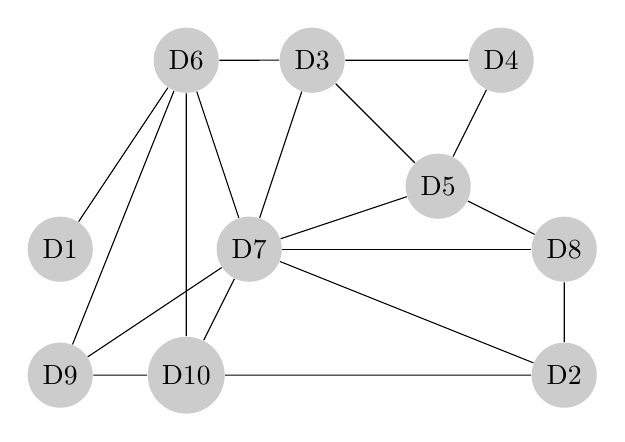
\begin{tikzpicture}
  [scale=.8,auto=left,every node/.style={circle,fill=black!20}]
  \node (n1) at (1,5) {D1};
  \node (n6) at (3,8)  {D6};
  \node (n3) at (5,8)  {D3};
  \node (n7) at (4,5)  {D7};
  \node (n9) at (1,3)  {D9};
  \node (n4) at (8,8)  {D4};
  \node (n5) at (7,6)  {D5};
  \node (n10) at (3,3) {D10};
  \node (n2) at (9,3)  {D2};
  \node (n8) at (9,5)  {D8};
  \foreach \from/\to in {n1/n6,n2/n7,n2/n8,n2/n10,n3/n6,n3/n7,n3/n4,n3/n5,n4/n5,n5/n8,n5/n7,n6/n7,n6/n9,n6/n10,n7/n9,n7/n10,n7/n8,n9/n10}
    \draw (\from) -- (\to);

\end{tikzpicture}
\\
Variables:      Domains\\
D1: District 1 \left\{ {blue, chartreuse, green,red}\right\} \\
D2: District 2 \left\{ {blue, chartreuse, green,red}\right\} \\
D3: District 3 \left\{ {blue, chartreuse, green,red}\right\} \\
D4: District 4 \left\{ {blue, chartreuse, green,red}\right\} \\
D5: District 5 \left\{ {blue, chartreuse, green,red}\right\} \\
D6: District 6 \left\{ {blue, chartreuse, green,red}\right\} \\
D7: District 7 \left\{ {blue, chartreuse, green,red}\right\} \\
D8: District 8 \left\{ {blue, chartreuse, green,red}\right\} \\
D9: District 9 \left\{ {blue, chartreuse, green,red}\right\} \\
D10: District 10 \left\{ {blue, chartreuse, green,red}\right\} \\




\end{document}
